% EE4525 2026 resit report. COMPULSORY STRUCTURE: exactly 8 pages, one item per page, this order.
% Every number comes from generated/*.tex (tools/evaluate.py --publish, tools/opvals.py, tools/report_extra.py).
% Never type a simulated number by hand. Build: latexmk (see report/README.md).
\documentclass[11pt,a4paper]{article}
\usepackage[margin=1.8cm]{geometry}
\usepackage{amsmath,amssymb}
\usepackage{booktabs,array,graphicx,float}
\usepackage[table]{xcolor}
\usepackage[font=small]{caption}
\usepackage{circuitikz}
\usetikzlibrary{calc,positioning}
\usepackage{xfp}
\usepackage{siunitx}
\usepackage[hidelinks]{hyperref}
\pagestyle{plain}
\setlength{\parindent}{0pt}
\setlength{\parskip}{4pt}

\IfFileExists{generated/results.tex}{% generated by tools/evaluate.py --publish; do not edit by hand
% tag final at 2026-10-05 23:28:41
\newcommand{\resSNR}{66.21}
\newcommand{\resAbeta}{66.76}
\newcommand{\resA}{81.59}
\newcommand{\resTsettle}{24.48}
\newcommand{\resTthirty}{13.913}
\newcommand{\resTthirtyeight}{15.704}
\newcommand{\resTau}{1.792}
\newcommand{\resPower}{0.2375}
\newcommand{\resIdd}{0.1320}
\newcommand{\resKTC}{323.80}
\newcommand{\resVnAmp}{360.33}
\newcommand{\resVnTot}{484.45}
\newcommand{\resVin}{350.00}
\newcommand{\resVout}{1.4000}
\newcommand{\resCin}{1.66}
\newcommand{\resCfb}{0.415}
\newcommand{\resCload}{1.66}
\newcommand{\resCCM}{0.05}
\newcommand{\resRbig}{0.4}
\newcommand{\resCbig}{10}
\newcommand{\resFoMlin}{6.403\times10^{-19}}
\newcommand{\resFoMdB}{181.94}
\newcommand{\resBetaIdeal}{0.2}
\newcommand{\resBetaActual}{0.1903}
\newcommand{\resGapdB}{14.41}
\newcommand{\resNEF}{6.241}
\newcommand{\resFirstPeak}{inf}
\newcommand{\resSlew}{1040}
\newcommand{\resCLeff}{1.992}
\newcommand{\resFoMEEtwenty}{175.2}
}{% placeholders until tools/evaluate.py --publish writes generated/results.tex (renders as red ??)
\providecommand{\resSNR}{\textcolor{red}{\textbf{??}}}
\providecommand{\resAbeta}{\textcolor{red}{\textbf{??}}}
\providecommand{\resA}{\textcolor{red}{\textbf{??}}}
\providecommand{\resTsettle}{\textcolor{red}{\textbf{??}}}
\providecommand{\resTthirty}{\textcolor{red}{\textbf{??}}}
\providecommand{\resTthirtyeight}{\textcolor{red}{\textbf{??}}}
\providecommand{\resTau}{\textcolor{red}{\textbf{??}}}
\providecommand{\resPower}{\textcolor{red}{\textbf{??}}}
\providecommand{\resIdd}{\textcolor{red}{\textbf{??}}}
\providecommand{\resKTC}{\textcolor{red}{\textbf{??}}}
\providecommand{\resVnAmp}{\textcolor{red}{\textbf{??}}}
\providecommand{\resVnTot}{\textcolor{red}{\textbf{??}}}
\providecommand{\resVin}{\textcolor{red}{\textbf{??}}}
\providecommand{\resVout}{\textcolor{red}{\textbf{??}}}
\providecommand{\resCin}{\textcolor{red}{\textbf{??}}}
\providecommand{\resCfb}{\textcolor{red}{\textbf{??}}}
\providecommand{\resCload}{\textcolor{red}{\textbf{??}}}
\providecommand{\resCCM}{\textcolor{red}{\textbf{??}}}
\providecommand{\resRbig}{\textcolor{red}{\textbf{??}}}
\providecommand{\resCbig}{\textcolor{red}{\textbf{??}}}
\providecommand{\resFoMlin}{\textcolor{red}{\textbf{??}}}
\providecommand{\resFoMdB}{\textcolor{red}{\textbf{??}}}
\providecommand{\resBetaIdeal}{\textcolor{red}{\textbf{??}}}
\providecommand{\resBetaActual}{\textcolor{red}{\textbf{??}}}
\providecommand{\resGapdB}{\textcolor{red}{\textbf{??}}}
\providecommand{\resNEF}{\textcolor{red}{\textbf{??}}}
\providecommand{\resFirstPeak}{\textcolor{red}{\textbf{??}}}
\providecommand{\resSlew}{\textcolor{red}{\textbf{??}}}
\providecommand{\resCLeff}{\textcolor{red}{\textbf{??}}}
\providecommand{\resFoMEEtwenty}{\textcolor{red}{\textbf{??}}}
}
\IfFileExists{generated/opvals.tex}{% generated by tools/opvals.py; do not edit by hand
\providecommand{\opV}[1]{\ifcsname opv@#1\endcsname\csname opv@#1\endcsname\else\textcolor{red}{\textbf{??\detokenize{#1}}}\fi}
\providecommand{\opI}[1]{\ifcsname opi@#1\endcsname\csname opi@#1\endcsname\else\textcolor{red}{\textbf{??\detokenize{#1}}}\fi}

\expandafter\def\csname opv@a1n\endcsname{1.222\,V}
\expandafter\def\csname opv@a1p\endcsname{1.222\,V}
\expandafter\def\csname opv@b1n\endcsname{0.273\,V}
\expandafter\def\csname opv@b1p\endcsname{0.273\,V}
\expandafter\def\csname opv@bn5\endcsname{0.272\,V}
\expandafter\def\csname opv@bp0\endcsname{1.434\,V}
\expandafter\def\csname opv@cmd\endcsname{0.590\,V}
\expandafter\def\csname opv@cmt\endcsname{1.511\,V}
\expandafter\def\csname opv@gp1\endcsname{1.200\,V}
\expandafter\def\csname opv@gp2\endcsname{1.200\,V}
\expandafter\def\csname opv@inn\endcsname{0.900\,V}
\expandafter\def\csname opv@inp\endcsname{0.900\,V}
\expandafter\def\csname opv@tail\endcsname{1.434\,V}
\expandafter\def\csname opv@vbn\endcsname{0.596\,V}
\expandafter\def\csname opv@vbnr\endcsname{0.596\,V}
\expandafter\def\csname opv@vbp\endcsname{1.200\,V}
\expandafter\def\csname opv@vbpr\endcsname{1.200\,V}
\expandafter\def\csname opv@vcmfb\endcsname{0.596\,V}
\expandafter\def\csname opv@vcmr\endcsname{0.900\,V}
\expandafter\def\csname opv@vcms\endcsname{0.896\,V}
\expandafter\def\csname opv@vcn\endcsname{0.916\,V}
\expandafter\def\csname opv@vcnr\endcsname{0.916\,V}
\expandafter\def\csname opv@vcp\endcsname{0.474\,V}
\expandafter\def\csname opv@vcpr\endcsname{0.474\,V}
\expandafter\def\csname opv@vdd\endcsname{1.800\,V}
\expandafter\def\csname opv@vddb\endcsname{1.800\,V}
\expandafter\def\csname opv@vin\endcsname{0.899\,V}
\expandafter\def\csname opv@vip\endcsname{0.899\,V}
\expandafter\def\csname opv@von\endcsname{0.896\,V}
\expandafter\def\csname opv@vop\endcsname{0.896\,V}
\expandafter\def\csname opv@x1n\endcsname{0.610\,V}
\expandafter\def\csname opv@x1p\endcsname{0.610\,V}
\expandafter\def\csname opv@zn\endcsname{0.896\,V}
\expandafter\def\csname opv@zp\endcsname{0.896\,V}
\expandafter\def\csname opi@cc1\endcsname{2.201e-16\,nA}
\expandafter\def\csname opi@cc2\endcsname{2.201e-16\,nA}
\expandafter\def\csname opi@ccm1\endcsname{2.479e-29\,nA}
\expandafter\def\csname opi@ccm2\endcsname{6.100e-29\,nA}
\expandafter\def\csname opi@cd1\endcsname{1.200e-11\,nA}
\expandafter\def\csname opi@cd2\endcsname{5.962e-12\,nA}
\expandafter\def\csname opi@cd3\endcsname{9.156e-12\,nA}
\expandafter\def\csname opi@cd4\endcsname{4.740e-12\,nA}
\expandafter\def\csname opi@cfb1\endcsname{1.770e-18\,nA}
\expandafter\def\csname opi@cfb2\endcsname{1.770e-18\,nA}
\expandafter\def\csname opi@cin1\endcsname{1.770e-18\,nA}
\expandafter\def\csname opi@cin2\endcsname{1.770e-18\,nA}
\expandafter\def\csname opi@cload1\endcsname{1.926e-15\,nA}
\expandafter\def\csname opi@cload2\endcsname{1.926e-15\,nA}
\expandafter\def\csname opi@cls1\endcsname{4.012e-16\,nA}
\expandafter\def\csname opi@cls2\endcsname{4.012e-16\,nA}
\expandafter\def\csname opi@ibcn\endcsname{38.40\,$\mu$A}
\expandafter\def\csname opi@ibcp\endcsname{25.60\,$\mu$A}
\expandafter\def\csname opi@ibnn\endcsname{6.400\,$\mu$A}
\expandafter\def\csname opi@ibnp\endcsname{6.400\,$\mu$A}
\expandafter\def\csname opi@m0\endcsname{115.2\,$\mu$A}
\expandafter\def\csname opi@m1\endcsname{57.60\,$\mu$A}
\expandafter\def\csname opi@m10\endcsname{74.39\,$\mu$A}
\expandafter\def\csname opi@m11\endcsname{74.39\,$\mu$A}
\expandafter\def\csname opi@m12\endcsname{74.39\,$\mu$A}
\expandafter\def\csname opi@m2\endcsname{57.60\,$\mu$A}
\expandafter\def\csname opi@m3\endcsname{57.60\,$\mu$A}
\expandafter\def\csname opi@m4\endcsname{57.60\,$\mu$A}
\expandafter\def\csname opi@m5\endcsname{57.60\,$\mu$A}
\expandafter\def\csname opi@m6\endcsname{57.60\,$\mu$A}
\expandafter\def\csname opi@m7\endcsname{51.20\,$\mu$A}
\expandafter\def\csname opi@m7c\endcsname{6.397\,$\mu$A}
\expandafter\def\csname opi@m8\endcsname{51.20\,$\mu$A}
\expandafter\def\csname opi@m8c\endcsname{6.397\,$\mu$A}
\expandafter\def\csname opi@m9\endcsname{74.39\,$\mu$A}
\expandafter\def\csname opi@mbn3\endcsname{38.40\,$\mu$A}
\expandafter\def\csname opi@mbn5\endcsname{6.400\,$\mu$A}
\expandafter\def\csname opi@mbn7\endcsname{6.400\,$\mu$A}
\expandafter\def\csname opi@mbp0\endcsname{6.400\,$\mu$A}
\expandafter\def\csname opi@mbp1\endcsname{6.400\,$\mu$A}
\expandafter\def\csname opi@mbp3\endcsname{25.60\,$\mu$A}
\expandafter\def\csname opi@mc0\endcsname{12.63\,$\mu$A}
\expandafter\def\csname opi@mc1\endcsname{6.517\,$\mu$A}
\expandafter\def\csname opi@mc2\endcsname{6.114\,$\mu$A}
\expandafter\def\csname opi@mc3\endcsname{6.517\,$\mu$A}
\expandafter\def\csname opi@mc4\endcsname{6.114\,$\mu$A}
\expandafter\def\csname opi@rb1\endcsname{0.000\,nA}
\expandafter\def\csname opi@rb2\endcsname{0.000\,nA}
\expandafter\def\csname opi@rcm1\endcsname{2.479e-10\,nA}
\expandafter\def\csname opi@rcm2\endcsname{6.100e-10\,nA}
\expandafter\def\csname opi@rd1\endcsname{2.220e-10\,nA}
\expandafter\def\csname opi@rd2\endcsname{0.000\,nA}
\expandafter\def\csname opi@rd3\endcsname{0.000\,nA}
\expandafter\def\csname opi@rd4\endcsname{0.000\,nA}
\expandafter\def\csname opi@rfb1\endcsname{0.008231\,nA}
\expandafter\def\csname opi@rfb2\endcsname{0.008231\,nA}
\expandafter\def\csname opi@rin1\endcsname{0.008231\,nA}
\expandafter\def\csname opi@rin2\endcsname{0.008231\,nA}
\expandafter\def\csname opi@rz1\endcsname{0.000\,nA}
\expandafter\def\csname opi@rz2\endcsname{0.000\,nA}
\expandafter\def\csname opi@vcmr\endcsname{0.000\,nA}
\expandafter\def\csname opi@vdd\endcsname{276.6\,$\mu$A}
\expandafter\def\csname opi@vddb\endcsname{76.80\,$\mu$A}
\expandafter\def\csname opi@vinn\endcsname{0.008231\,nA}
\expandafter\def\csname opi@vinp\endcsname{0.008231\,nA}
}{%
  \providecommand{\opV}[1]{\textcolor{red}{\textbf{??}}}\providecommand{\opI}[1]{\textcolor{red}{\textbf{??}}}}
\IfFileExists{generated/extra.tex}{% generated by tools/report_extra.py; do not edit by hand
% from results/final/summary.json
\newcommand{\xFc}{34.8}
\newcommand{\xPM}{80.1}
\newcommand{\xGM}{nan}
\newcommand{\xTzero}{81.1}
\newcommand{\xTzeroExt}{76.5}
\newcommand{\xFcExt}{34.4}
\newcommand{\xPMExt}{79.9}
\newcommand{\xTauWc}{4.58}
\newcommand{\xTauTwoPole}{3.47}
\newcommand{\xCMfc}{7.6}
\newcommand{\xCMpm}{82}
\newcommand{\xCMtzero}{29.3}
\newcommand{\xCMexc}{18.5}
\newcommand{\xCMexcT}{4.6}
\newcommand{\xCMexcTf}{3.6}
\newcommand{\xVcm}{0.896}
\newcommand{\xTauSmall}{2.59}
\newcommand{\xTthirtySmall}{12.3}
\newcommand{\xTauMid}{2.20}
\newcommand{\xTauExact}{2.5004}
\newcommand{\xXswing}{170}
\newcommand{\xGpswing}{131}
\newcommand{\xIpk}{220}
\newcommand{\xOvershoot}{20}
\newcommand{\xOvershootFinal}{156}
\newcommand{\xOvershootT}{28.3}
\newcommand{\xTauWforty}{2.18}
\newcommand{\xTauWfifty}{1.86}
\newcommand{\xAbEnd}{78.9}
\newcommand{\xAEnd}{93.8}
\newcommand{\xGapEnd}{14.9}
\newcommand{\xTend}{70}
\newcommand{\xAbLong}{79.0}
\newcommand{\xOutMarg}{156}
\newcommand{\xOutDev}{M_{11}}
\newcommand{\xEKTC}{183}
\newcommand{\xESNR}{72.60}
\newcommand{\xEFoMspec}{175.20}
\newcommand{\xEFoMach}{175.41}
\newcommand{\xEFoM}{167.17}
\newcommand{\xDP}{-6.87}
\newcommand{\xDT}{+22.99}
\newcommand{\xDS}{-6.41}
\newcommand{\xDTot}{+9.71}
\newcommand{\xDNet}{+5.41}
\newcommand{\xDBeta}{+2.55}
\newcommand{\xDShape}{+1.43}
\newcommand{\xDShare}{-2.59}
\newcommand{\xDSwing}{+0.00}
\newcommand{\xDAmp}{+2.91}
\newcommand{\xShareNow}{47}
\newcommand{\xShareEE}{85}
\newcommand{\xPratio}{4.87}
\newcommand{\xTauRatio}{199}
\newcommand{\xCapRatio}{8.4}
\newcommand{\xPTauOld}{55659.1}
\newcommand{\xStepMarg}{94}
\newcommand{\xStepDev}{M_{7}}
\newcommand{\xQMarg}{94}
\newcommand{\xQDev}{M_{BN7}}
\newcommand{\xIq}{276.6}
\newcommand{\xIwin}{302.6}
\newcommand{\xIslew}{26.0}
\newcommand{\xNshIn}{51}
\newcommand{\xNshLoad}{36}
\newcommand{\xNshCasc}{0}
\newcommand{\xNshRz}{8}
\newcommand{\xNshStTwo}{5}
\newcommand{\xNshRb}{0.1}
\newcommand{\xNshCmfb}{0.0}
\newcommand{\xNin}{153}
\newcommand{\xNload}{121}
\newcommand{\xNrz}{59}
\newcommand{\xFlickUV}{81}
\newcommand{\xFlickShare}{7}
\newcommand{\xFlickIn}{31}
\newcommand{\xFlickLoad}{38}
\newcommand{\xIdIn}{57.6}
\newcommand{\xGmOne}{0.961}
\newcommand{\xGmIdIn}{16.7}
\newcommand{\xIdTwo}{74.4}
\newcommand{\xGmNine}{0.829}
\newcommand{\xGmEleven}{0.812}
\newcommand{\xGmIdNine}{11.1}
\newcommand{\xGmIdEleven}{10.9}
\newcommand{\xCp}{64}
\newcommand{\xFoMideal}{178.8}
\newcommand{\xFoMone}{177.06}
\newcommand{\xLcur}{-4.19}
\newcommand{\xEtaCur}{38}
\newcommand{\xLnoise}{-3.29}
\newcommand{\xGtau}{+7.29}
\newcommand{\xTauOne}{13.4}
\newcommand{\pIbnp}{6.40}
\newcommand{\pN}{9}
\newcommand{\pNcm}{1}
\newcommand{\pMtwo}{11}
\newcommand{\pMcmt}{2}
\newcommand{\pKcn}{6.00}
\newcommand{\pKcp}{4.00}
\newcommand{\pRd}{1}
\newcommand{\pCc}{0.770}
\newcommand{\pRz}{2.37}
\newcommand{\pCls}{0.68}
\newcommand{\pRb}{2}
\newcommand{\pRcm}{2}
\newcommand{\pCcm}{50}
\newcommand{\pVcmi}{0.90}
\newcommand{\pLl}{2.0}
\newcommand{\pLi}{0.18}
\newcommand{\pLt}{0.5}
\newcommand{\pLd}{0.25}
}{}
% Shared CircuiTikZ style for the D2/D3 figures (input by main.tex).
% One drawing per block serves both sheets: \showIfalse = node voltages (D2), \showItrue = currents (D3).
%   \Vtag{node}   blue node voltage from generated/opvals.tex  (LTspice node name, lower case)
%   \Itag{device} red branch current from generated/opvals.tex  (device name, lower case)
\ctikzset{bipoles/length=1.0cm, transistors/arrow pos=end, transistors/scale=0.8}
\tikzset{every picture/.append style={line cap=round, line join=round, line width=0.6pt}}
\newif\ifshowI \showIfalse
\newcommand{\Vtag}[1]{\ifshowI\else\textcolor{blue!60!black}{\footnotesize\opV{#1}}\fi}
\newcommand{\Itag}[1]{\ifshowI\textcolor{red!65!black}{\footnotesize\opI{#1}}\fi}

% EE4520 baseline (reference/ee4520/: P, tau and achieved SNR as reported there)
\newcommand{\ePow}{0.1119}\newcommand{\eTau}{497.4}\newcommand{\eSNR}{80.85}
\newcommand{\dB}[1]{\fpeval{round(10*ln(#1)/ln(10),2)}}
\newcommand{\dd}[2][2]{\edef\ddtmp{\fpeval{#2}}\num[round-mode=places,round-precision=#1]{\ddtmp}}
\newcommand{\lgt}[1]{(ln(#1)/ln(10))}
% EE4520 like-for-like: kT/C of its gain-8 network (Cin = Cload = 18 pF, Cfb = 2.25 pF) with the EE4525 rule
\newcommand{\eKTC}{(sqrt(2*1.380649e-23*300.15*(18e-12/(2.25e-12)^2 + 1/2.25e-12 + 1/18e-12)))}
\newcommand{\eSNRll}{(20*\lgt{0.8485/sqrt((76.93e-6)^2 + \eKTC^2)})}
\newcommand{\eFoM}[1]{((#1) - 10*\lgt{2*pi*\ePow e-3*\eTau e-9})}

\begin{document}

%% ---------------------------------------------------------------- page 1: title
\begin{titlepage}
  \centering
  \vspace*{5cm}
  {\Large Delft University of Technology\par}
  \vspace{1.5cm}
  {\huge\bfseries Analogue CMOS Design II\par}
  \vspace{0.4cm}
  {\Large A Residue Amplifier for a Pipeline ADC\par}
  \vspace{0.4cm}
  {\Large EE4525 2026\par}
  \vspace{2cm}
  {\Large Daniel Tyukov\par}
  {\large Student number: 5714699\par}
  \vfill
  {\large \today\par}
\end{titlepage}
\setcounter{page}{2}

%% ---------------------------------------------------------------- page 2: D1
\section*{Deliverable 1: Table of Results}
\begin{table}[H]
\centering
\renewcommand{\arraystretch}{1.18}\setlength{\tabcolsep}{5pt}
\begin{tabular}{r l c c r}
\toprule
Item & Design item & Unit & Spec. & Achieved \\
\midrule
1  & SNR & dB & 66 & \resSNR \\
2  & $A\beta_{settle}$ (loop settling) & dB & 66 & \resAbeta \\
3  & $A_{settle}$ (amplifier settling) & dB & $>78$ & \resA \\
4  & $T_{settle}$ (settling time to required accuracy) & ns & 25 & \resTsettle \\
5  & $T_{30\,\mathrm{dB}}$ & ns & - & \resTthirty \\
6  & $T_{38.6\,\mathrm{dB}}$ & ns & - & \resTthirtyeight \\
7  & $\tau = T_{38.6\,\mathrm{dB}} - T_{30\,\mathrm{dB}}$ & ns & - & \resTau \\
8  & Power dissipation (amplifiers only) & mW & $<3$, as low as possible & \resPower \\
9  & $I(V_{dd})$ (amplifiers only, no biasing) & mA & $<1.7$, as low as possible & \resIdd \\
10 & Total effective $kT/C$ noise at output & $\mu$V$_{\mathrm{rms}}$ & free & \resKTC \\
11 & Total integrated amplifier noise & $\mu$V$_{\mathrm{rms}}$ & free & \resVnAmp \\
12 & Total integrated noise (10\,kHz to 100\,GHz) & $\mu$V$_{\mathrm{rms}}$ & free & \resVnTot \\
13 & Input step voltage & mV & Output/4 & \resVin \\
14 & Output step voltage & V & free & \resVout \\
15 & $C_{in}$ & pF & - & \resCin \\
16 & $C_{fb}$ & pF & - & \resCfb \\
17 & $C_{load}$ & pF & $= C_{in}$ & \resCload \\
18 & $C_{CM}$ & pF & - & \resCCM \\
19 & $R_{fb}$ & G$\Omega$ & big & \resRbig \\
20 & $C_{big}$ & nF & big & \resCbig \\
21 & $\mathrm{FoM_{lin}} = 2\pi \cdot \mathrm{Power}\cdot\tau/\mathrm{SNR_{lin}}^2$ & J & $<9.5\times10^{-18}$ & $\resFoMlin$ \\
22 & $\mathrm{FoM_{dB}} = -10\log_{10}(\mathrm{FoM_{lin}})$ & dB & $>170$ & \resFoMdB \\
\bottomrule
\end{tabular}
\end{table}
\small
Both steps are differential: $\resVin$\,mV in, $\fpeval{round(\resVout,2)}$\,V peak out, so each output swings
$0.9 \pm \fpeval{\resVout/2}$\,V. I report power as 1.8\,V times the larger of two averages of $I(V_{dd})$: the quiescent
one and the one over the 25\,ns after the step. The second is higher here (\xIwin\,$\mu$A against \xIq\,$\mu$A) because
the class-AB output takes the load charge from $V_{dd}$ during the step. The bias block runs from its own $V_{ddb}$ and is
not counted. The $kT/C$ noise is $v_{n}^2 = 42\,kT/C_{in}$ (differential, from $C_{in}$, $C_{fb}$ and $C_{load}$ only,
$T = 300.15$\,K). The amplifier noise is the \texttt{.noise} result for $V(v_{on},v_{op})$ integrated from 10\,kHz to
100\,GHz, with $R_{in} = 100$\,M$\Omega$ and $R_{fb} = 400$\,M$\Omega$ set \texttt{noiseless} as the FAQ allows. $C_{CM}$
is the CMFB sense capacitor on each side, in parallel with a 2\,M$\Omega$ resistor. $\tau$ is one $e$-fold (8.6\,dB) of the
$A\beta$ curve.
\normalsize
\clearpage

%% ---------------------------------------------------------------- page 3: D2
\section*{Deliverable 2: Schematic with Node Voltages}
\showIfalse
\begin{figure}[H]\centering
\resizebox{\linewidth}{!}{% TODO(agent): replace with the real amplifier drawing (CircuiTikZ, readable, all nodes/branches tagged).
% Example of the tagging pattern on a differential pair (names must match the LTspice netlist):
\begin{circuitikz}[american]
  \draw (0,0) node[nmos](M1){} (3,0) node[nmos, xscale=-1](M2){};
  \draw (M1.S) -- ++(0,-0.5) coordinate(t) -| (M2.S);
  \draw (t) node[below]{\Vtag{tail}};
  \draw (M1.D) node[above]{\Vtag{von}\ \Itag{m1}};
  \draw (M2.D) node[above]{\Vtag{vop}\ \Itag{m2}};
  \draw (M1.G) node[left]{$v_{ip}$} (M2.G) node[right]{$v_{in}$};
\end{circuitikz}
}
\caption{Amplifier core (stage 1, class-AB stage 2, current-buffer compensation) with DC node voltages
(operating point, no input step). $V_{DD} = 1.8$\,V. Bulks: NMOS to ground, input and CMFB pairs to their
own source, other PMOS to $V_{DD}$.}
\end{figure}
\vspace{-4mm}
\begin{figure}[H]\centering
\begin{minipage}[b]{0.47\linewidth}\centering
\resizebox{\linewidth}{!}{% CMFB: resistive output-CM sense (Rcm || Ccm), PMOS pair against vcmr, diode loads; vcmfb drives M7C, M8C.
\begin{circuitikz}[american, scale=0.85]
\small
\draw (0,0) node[left]{$v_{op}$} to[R, l_={$R_{cm}$}, o-*] (2.6,0);
\draw (0,-2.6) node[left]{$v_{on}$} to[R, l={$R_{cm}$}, o-*] (2.6,-2.6);
\draw (0.35,0) node[circ]{} -- (0.35,0.9) to[C, l={$C_{CM}$}] (2.25,0.9) -- (2.25,0);
\draw (0.35,-2.6) node[circ]{} -- (0.35,-3.5) to[C, l_={$C_{CM}$}] (2.25,-3.5) -- (2.25,-2.6);
\draw (2.6,0) -- (2.6,-2.6);
\draw (2.6,-1.3) node[circ]{} coordinate(vcms);
\draw (6.65,1.0) node[pmos](MC0){};
\draw (MC0.S) -- ++(0,0.25) node[vdd]{};
\draw (MC0.G) -- ++(-0.3,0) node[left]{$v_{bp}$};
\draw (MC0.D) -- (6.65,0.1) coordinate(cmt);
\draw (4.4,0.1) -- (8.9,0.1);
\draw (4.4,-1.3) node[pmos](MC1){};
\draw (8.9,-1.3) node[pmos,xscale=-1](MC2){};
\draw (MC1.S) -- (4.4,0.1) (MC2.S) -- (8.9,0.1);
\draw (vcms) -- (MC1.G);
\draw (MC2.G) -- ++(0.3,0) node[right]{$v_{cmr}$};
\draw (4.4,-3.9) node[nmos](MC3){};
\draw (8.9,-3.9) node[nmos,xscale=-1](MC4){};
\draw (MC1.D) -- (MC3.D) (MC2.D) -- (MC4.D);
\draw (MC3.S) node[ground]{} (MC4.S) node[ground]{};
\draw (MC3.G) -- ++(-0.3,0) |- (4.4,-2.75) node[circ]{};
\draw (MC4.G) -- ++(0.3,0) |- (8.9,-2.75) node[circ]{} coordinate(cmd);
\draw (4.4,-2.35) node[circ]{} -- (3.0,-2.35) |- (2.6,-4.7) node[left]{$v_{cmfb}\to M_{7C}, M_{8C}$};
\node[font=\small,anchor=south east] at (vcms) {$v_{cms}$\,\Vtag{vcms}};
\node[font=\small,anchor=south west] at ($(cmt)+(0.05,0)$) {$n_{cmt}$\,\Vtag{cmt}};
\ifshowI\else\node[font=\small,anchor=south west,align=left] at ($(2.72,-2.35)$) {$v_{cmfb}$\\\Vtag{vcmfb}};\fi
\node[font=\small,anchor=south west] at (cmd) {$n_{cmd}$\,\Vtag{cmd}};
\node[font=\small,anchor=west] at ($(MC2.G)+(0.3,-0.4)$) {\Vtag{vcmr}};
\def\dl#1#2#3{\node[anchor=west,font=\small,align=left] at ($(#1.center)+(0.42,0.1)$) {#2\\\Itag{#3}};}
\def\dr#1#2#3{\node[anchor=east,font=\small,align=right] at ($(#1.center)+(-0.42,0.1)$) {#2\\\Itag{#3}};}
\dl{MC0}{$M_{C0}$}{mc0} \dl{MC1}{$M_{C1}$}{mc1} \dr{MC2}{$M_{C2}$}{mc2} \dl{MC3}{$M_{C3}$}{mc3} \dr{MC4}{$M_{C4}$}{mc4}
\end{circuitikz}
}
\caption{CMFB with node voltages.}
\end{minipage}\hfill
\begin{minipage}[b]{0.5\linewidth}\centering
\resizebox{\linewidth}{!}{% Bias block on Vddb (excluded from the amplifier power). Replica of one stage-1 half circuit: the P replica
% (tail unit + input unit with its gate at vcmr) sets vbp, the N replica (NMOS cascode unit + load unit) sets vbn.
% vcn and vcp come from diodes fed by fixed multiples of Ibnp (EE4520 fig. 6). Every line: Rd + Cbig.
\begin{circuitikz}[american, scale=0.8]
\small
\def\dn#1#2#3#4{\node[anchor=#4,font=\footnotesize,align=center] at #1 {#2\\\Itag{#3}};}
% ---- P replica (top left): MBP0 tail unit (gate from the input unit's drain), MBP1 input unit, Ibnp sink
\draw (0,0) node[pmos,xscale=-1](BP0){};
\draw (BP0.S) -- ++(0,0.25) node[vdd]{};
\draw (0,-1.8) node[pmos](BP1){};
\draw (BP0.D) -- (BP1.S) coordinate[midway](bp0);
\draw (BP1.G) -- ++(-0.3,0) node[left]{$v_{cmr}$};
\draw (BP1.D) -- (0,-3.0) coordinate(vbpr) to[I, l_={$I_{bnp}$}] (0,-4.6) node[ground]{};
\draw (BP0.G) -- (2.7,0 |- BP0.G) -- (2.7,-3.0) -- (vbpr) node[circ]{};
\draw (2.7,-3.0) node[circ]{} to[R, l_={$R_d$}] (4.3,-3.0) node[circ]{} coordinate(ovbp) to[C, l={$C_{big}$}] (4.3,-4.6) node[ground]{};
\node[anchor=south west,font=\small] at (ovbp) {$v_{bp}$\,\Vtag{vbp}};
\node[anchor=east,font=\footnotesize] at ($(bp0)+(-0.1,0)$) {$b_{p0}$\,\Vtag{bp0}};
\dn{($(BP0.center)+(-1.15,0.15)$)}{$M_{BP0}$}{mbp0}{east}
\dn{($(BP1.center)+(0.55,-0.1)$)}{$M_{BP1}$}{mbp1}{west}
% ---- N replica (top right): Ibnp from Vddb, MBN5 cascode unit (gate vcn), MBN7 load unit (gate from the top)
\draw (9.2,-1.4) node[nmos](BN5){};
\draw (9.2,-3.4) node[nmos,xscale=-1](BN7){};
\draw (BN5.D) -- (9.2,-0.5) coordinate(vbnr) to[I, l={$I_{bnp}$}, invert] (9.2,1.1) node[vdd]{};
\draw (BN5.S) -- (BN7.D) coordinate[midway](bn5);
\draw (BN5.G) -- ++(-0.3,0) node[left]{$v_{cn}$};
\draw (BN7.S) node[ground]{};
\draw (BN7.G) -- (10.6,0 |- BN7.G) -- (10.6,-0.5) -- (vbnr) node[circ]{};
\draw (10.6,-0.5) node[circ]{} to[R, l_={$R_d$}] (12.5,-0.5) node[circ]{} coordinate(ovbn) to[C, l={$C_{big}$}] (12.5,-2.1) node[ground]{};
\node[anchor=south west,font=\small] at (ovbn) {$v_{bn}$\,\Vtag{vbn}};
\node[anchor=east,font=\footnotesize] at ($(bn5)+(-0.1,0)$) {$b_{n5}$\,\Vtag{bn5}};
\dn{($(BN5.center)+(-0.75,0.85)$)}{$M_{BN5}$}{mbn5}{east}
\dn{($(BN7.center)+(-0.55,-0.85)$)}{$M_{BN7}$}{mbn7}{east}
% ---- vcn (bottom left): diode MBN3 fed by kcn Ibnp
\draw (0,-9.0) node[nmos,xscale=-1](BN3){};
\draw (BN3.D) -- (0,-8.0) coordinate(vcnr) to[I, l={$k_{cn}I_{bnp}$}, invert] (0,-6.4) node[vdd]{};
\draw (BN3.S) node[ground]{};
\draw (BN3.G) -- (2.7,0 |- BN3.G) -- (2.7,-8.0) -- (vcnr) node[circ]{};
\draw (2.7,-8.0) node[circ]{} to[R, l_={$R_d$}] (4.3,-8.0) node[circ]{} coordinate(ovcn) to[C, l={$C_{big}$}] (4.3,-9.6) node[ground]{};
\node[anchor=south west,font=\small] at (ovcn) {$v_{cn}$\,\Vtag{vcn}};
\dn{($(BN3.center)+(-0.55,-0.2)$)}{$M_{BN3}$}{mbn3}{east}
% ---- vcp (bottom right): diode MBP3 sinking kcp Ibnp
\draw (9.2,-7.1) node[pmos,xscale=-1](BP3){};
\draw (BP3.S) -- ++(0,0.25) node[vdd]{};
\draw (BP3.D) -- (9.2,-8.1) coordinate(vcpr) to[I, l_={$k_{cp}I_{bnp}$}] (9.2,-9.7) node[ground]{};
\draw (BP3.G) -- (10.6,0 |- BP3.G) -- (10.6,-8.1) -- (vcpr) node[circ]{};
\draw (10.6,-8.1) node[circ]{} to[R, l_={$R_d$}] (12.5,-8.1) node[circ]{} coordinate(ovcp) to[C, l={$C_{big}$}] (12.5,-9.7) node[ground]{};
\node[anchor=south west,font=\small] at (ovcp) {$v_{cp}$\,\Vtag{vcp}};
\dn{($(BP3.center)+(-1.15,0.15)$)}{$M_{BP3}$}{mbp3}{east}
\node[font=\footnotesize,align=left,anchor=north west] at (-1.6,-10.5) {supply arrows: $V_{ddb}$;
$I_{bnp} = \pIbnp\,\mu$A, $k_{cn} = \pKcn$, $k_{cp} = \pKcp$\\$R_d = \pRd$\,k$\Omega$, $C_{big} = \resCbig$\,nF};
\end{circuitikz}
}
\caption{Bias block on $V_{ddb} = 1.8$\,V with bias-line voltages.}
\end{minipage}
\end{figure}
\clearpage

%% ---------------------------------------------------------------- page 4: D3
\section*{Deliverable 3: Schematic with Branch Currents}
\showItrue
\begin{figure}[H]\centering
\resizebox{\linewidth}{!}{% TODO(agent): replace with the real amplifier drawing (CircuiTikZ, readable, all nodes/branches tagged).
% Example of the tagging pattern on a differential pair (names must match the LTspice netlist):
\begin{circuitikz}[american]
  \draw (0,0) node[nmos](M1){} (3,0) node[nmos, xscale=-1](M2){};
  \draw (M1.S) -- ++(0,-0.5) coordinate(t) -| (M2.S);
  \draw (t) node[below]{\Vtag{tail}};
  \draw (M1.D) node[above]{\Vtag{von}\ \Itag{m1}};
  \draw (M2.D) node[above]{\Vtag{vop}\ \Itag{m2}};
  \draw (M1.G) node[left]{$v_{ip}$} (M2.G) node[right]{$v_{in}$};
\end{circuitikz}
}
\caption{Amplifier core with DC drain currents of every transistor (red). Stage 1 is one current path per side:
$M_{tp} \to M_{1p} \to M_{cp} \to M_{cn} \to M_{1n} \to M_{tn}+M_{tc}$ (current reuse).}
\end{figure}
\vspace{-4mm}
\begin{figure}[H]\centering
\begin{minipage}[b]{0.47\linewidth}\centering
\resizebox{\linewidth}{!}{% CMFB: resistive output-CM sense (Rcm || Ccm), PMOS pair against vcmr, diode loads; vcmfb drives M7C, M8C.
\begin{circuitikz}[american, scale=0.85]
\small
\draw (0,0) node[left]{$v_{op}$} to[R, l_={$R_{cm}$}, o-*] (2.6,0);
\draw (0,-2.6) node[left]{$v_{on}$} to[R, l={$R_{cm}$}, o-*] (2.6,-2.6);
\draw (0.35,0) node[circ]{} -- (0.35,0.9) to[C, l={$C_{CM}$}] (2.25,0.9) -- (2.25,0);
\draw (0.35,-2.6) node[circ]{} -- (0.35,-3.5) to[C, l_={$C_{CM}$}] (2.25,-3.5) -- (2.25,-2.6);
\draw (2.6,0) -- (2.6,-2.6);
\draw (2.6,-1.3) node[circ]{} coordinate(vcms);
\draw (6.65,1.0) node[pmos](MC0){};
\draw (MC0.S) -- ++(0,0.25) node[vdd]{};
\draw (MC0.G) -- ++(-0.3,0) node[left]{$v_{bp}$};
\draw (MC0.D) -- (6.65,0.1) coordinate(cmt);
\draw (4.4,0.1) -- (8.9,0.1);
\draw (4.4,-1.3) node[pmos](MC1){};
\draw (8.9,-1.3) node[pmos,xscale=-1](MC2){};
\draw (MC1.S) -- (4.4,0.1) (MC2.S) -- (8.9,0.1);
\draw (vcms) -- (MC1.G);
\draw (MC2.G) -- ++(0.3,0) node[right]{$v_{cmr}$};
\draw (4.4,-3.9) node[nmos](MC3){};
\draw (8.9,-3.9) node[nmos,xscale=-1](MC4){};
\draw (MC1.D) -- (MC3.D) (MC2.D) -- (MC4.D);
\draw (MC3.S) node[ground]{} (MC4.S) node[ground]{};
\draw (MC3.G) -- ++(-0.3,0) |- (4.4,-2.75) node[circ]{};
\draw (MC4.G) -- ++(0.3,0) |- (8.9,-2.75) node[circ]{} coordinate(cmd);
\draw (4.4,-2.35) node[circ]{} -- (3.0,-2.35) |- (2.6,-4.7) node[left]{$v_{cmfb}\to M_{7C}, M_{8C}$};
\node[font=\small,anchor=south east] at (vcms) {$v_{cms}$\,\Vtag{vcms}};
\node[font=\small,anchor=south west] at ($(cmt)+(0.05,0)$) {$n_{cmt}$\,\Vtag{cmt}};
\ifshowI\else\node[font=\small,anchor=south west,align=left] at ($(2.72,-2.35)$) {$v_{cmfb}$\\\Vtag{vcmfb}};\fi
\node[font=\small,anchor=south west] at (cmd) {$n_{cmd}$\,\Vtag{cmd}};
\node[font=\small,anchor=west] at ($(MC2.G)+(0.3,-0.4)$) {\Vtag{vcmr}};
\def\dl#1#2#3{\node[anchor=west,font=\small,align=left] at ($(#1.center)+(0.42,0.1)$) {#2\\\Itag{#3}};}
\def\dr#1#2#3{\node[anchor=east,font=\small,align=right] at ($(#1.center)+(-0.42,0.1)$) {#2\\\Itag{#3}};}
\dl{MC0}{$M_{C0}$}{mc0} \dl{MC1}{$M_{C1}$}{mc1} \dr{MC2}{$M_{C2}$}{mc2} \dl{MC3}{$M_{C3}$}{mc3} \dr{MC4}{$M_{C4}$}{mc4}
\end{circuitikz}
}
\caption{CMFB with branch currents.}
\end{minipage}\hfill
\begin{minipage}[b]{0.5\linewidth}\centering
\resizebox{\linewidth}{!}{% Bias block on Vddb (excluded from the amplifier power). Replica of one stage-1 half circuit: the P replica
% (tail unit + input unit with its gate at vcmr) sets vbp, the N replica (NMOS cascode unit + load unit) sets vbn.
% vcn and vcp come from diodes fed by fixed multiples of Ibnp (EE4520 fig. 6). Every line: Rd + Cbig.
\begin{circuitikz}[american, scale=0.8]
\small
\def\dn#1#2#3#4{\node[anchor=#4,font=\footnotesize,align=center] at #1 {#2\\\Itag{#3}};}
% ---- P replica (top left): MBP0 tail unit (gate from the input unit's drain), MBP1 input unit, Ibnp sink
\draw (0,0) node[pmos,xscale=-1](BP0){};
\draw (BP0.S) -- ++(0,0.25) node[vdd]{};
\draw (0,-1.8) node[pmos](BP1){};
\draw (BP0.D) -- (BP1.S) coordinate[midway](bp0);
\draw (BP1.G) -- ++(-0.3,0) node[left]{$v_{cmr}$};
\draw (BP1.D) -- (0,-3.0) coordinate(vbpr) to[I, l_={$I_{bnp}$}] (0,-4.6) node[ground]{};
\draw (BP0.G) -- (2.7,0 |- BP0.G) -- (2.7,-3.0) -- (vbpr) node[circ]{};
\draw (2.7,-3.0) node[circ]{} to[R, l_={$R_d$}] (4.3,-3.0) node[circ]{} coordinate(ovbp) to[C, l={$C_{big}$}] (4.3,-4.6) node[ground]{};
\node[anchor=south west,font=\small] at (ovbp) {$v_{bp}$\,\Vtag{vbp}};
\node[anchor=east,font=\footnotesize] at ($(bp0)+(-0.1,0)$) {$b_{p0}$\,\Vtag{bp0}};
\dn{($(BP0.center)+(-1.15,0.15)$)}{$M_{BP0}$}{mbp0}{east}
\dn{($(BP1.center)+(0.55,-0.1)$)}{$M_{BP1}$}{mbp1}{west}
% ---- N replica (top right): Ibnp from Vddb, MBN5 cascode unit (gate vcn), MBN7 load unit (gate from the top)
\draw (9.2,-1.4) node[nmos](BN5){};
\draw (9.2,-3.4) node[nmos,xscale=-1](BN7){};
\draw (BN5.D) -- (9.2,-0.5) coordinate(vbnr) to[I, l={$I_{bnp}$}, invert] (9.2,1.1) node[vdd]{};
\draw (BN5.S) -- (BN7.D) coordinate[midway](bn5);
\draw (BN5.G) -- ++(-0.3,0) node[left]{$v_{cn}$};
\draw (BN7.S) node[ground]{};
\draw (BN7.G) -- (10.6,0 |- BN7.G) -- (10.6,-0.5) -- (vbnr) node[circ]{};
\draw (10.6,-0.5) node[circ]{} to[R, l_={$R_d$}] (12.5,-0.5) node[circ]{} coordinate(ovbn) to[C, l={$C_{big}$}] (12.5,-2.1) node[ground]{};
\node[anchor=south west,font=\small] at (ovbn) {$v_{bn}$\,\Vtag{vbn}};
\node[anchor=east,font=\footnotesize] at ($(bn5)+(-0.1,0)$) {$b_{n5}$\,\Vtag{bn5}};
\dn{($(BN5.center)+(-0.75,0.85)$)}{$M_{BN5}$}{mbn5}{east}
\dn{($(BN7.center)+(-0.55,-0.85)$)}{$M_{BN7}$}{mbn7}{east}
% ---- vcn (bottom left): diode MBN3 fed by kcn Ibnp
\draw (0,-9.0) node[nmos,xscale=-1](BN3){};
\draw (BN3.D) -- (0,-8.0) coordinate(vcnr) to[I, l={$k_{cn}I_{bnp}$}, invert] (0,-6.4) node[vdd]{};
\draw (BN3.S) node[ground]{};
\draw (BN3.G) -- (2.7,0 |- BN3.G) -- (2.7,-8.0) -- (vcnr) node[circ]{};
\draw (2.7,-8.0) node[circ]{} to[R, l_={$R_d$}] (4.3,-8.0) node[circ]{} coordinate(ovcn) to[C, l={$C_{big}$}] (4.3,-9.6) node[ground]{};
\node[anchor=south west,font=\small] at (ovcn) {$v_{cn}$\,\Vtag{vcn}};
\dn{($(BN3.center)+(-0.55,-0.2)$)}{$M_{BN3}$}{mbn3}{east}
% ---- vcp (bottom right): diode MBP3 sinking kcp Ibnp
\draw (9.2,-7.1) node[pmos,xscale=-1](BP3){};
\draw (BP3.S) -- ++(0,0.25) node[vdd]{};
\draw (BP3.D) -- (9.2,-8.1) coordinate(vcpr) to[I, l_={$k_{cp}I_{bnp}$}] (9.2,-9.7) node[ground]{};
\draw (BP3.G) -- (10.6,0 |- BP3.G) -- (10.6,-8.1) -- (vcpr) node[circ]{};
\draw (10.6,-8.1) node[circ]{} to[R, l_={$R_d$}] (12.5,-8.1) node[circ]{} coordinate(ovcp) to[C, l={$C_{big}$}] (12.5,-9.7) node[ground]{};
\node[anchor=south west,font=\small] at (ovcp) {$v_{cp}$\,\Vtag{vcp}};
\dn{($(BP3.center)+(-1.15,0.15)$)}{$M_{BP3}$}{mbp3}{east}
\node[font=\footnotesize,align=left,anchor=north west] at (-1.6,-10.5) {supply arrows: $V_{ddb}$;
$I_{bnp} = \pIbnp\,\mu$A, $k_{cn} = \pKcn$, $k_{cp} = \pKcp$\\$R_d = \pRd$\,k$\Omega$, $C_{big} = \resCbig$\,nF};
\end{circuitikz}
}
\caption{Bias block (reference currents, $V_{ddb}$).}
\end{minipage}
\end{figure}
\clearpage

%% ---------------------------------------------------------------- page 5: D4
\section*{Deliverable 4: Plot of Settling Behaviour}
\begin{figure}[H]\centering
\IfFileExists{figures/d4_settling.pdf}{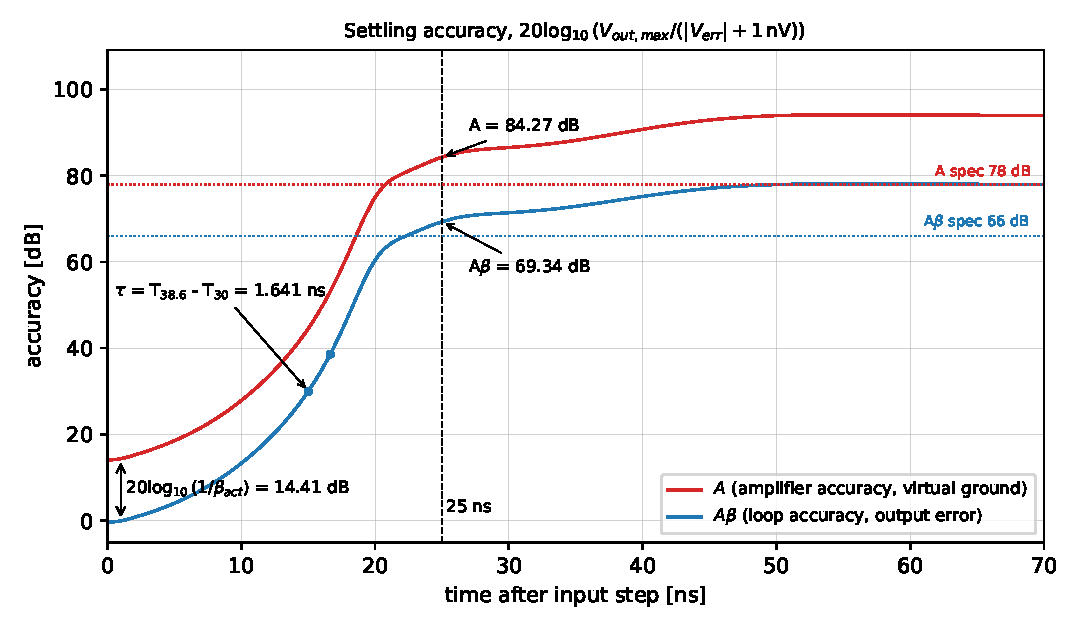
\includegraphics[width=\linewidth]{figures/d4_settling.pdf}}{\textcolor{red}{\textbf{?? missing figures/d4\_settling.pdf}}}
\caption{Settling accuracy versus time after the input step: $A$ (red, from the virtual-ground error
$|V(v_{ip})-V(v_{in})|$) and $A\beta$ (blue, from the output error $|V_{out,step}-V(v_{on},v_{op})|$, starting at 0\,dB),
both relative to $V_{out,step} = \resVout$\,V. At 25\,ns: $A = \resA$\,dB, $A\beta = \resAbeta$\,dB; settled to
both specifications at $\resTsettle$\,ns; $\tau = \resTau$\,ns.}
\end{figure}
\clearpage

%% ---------------------------------------------------------------- page 6: D5
\section*{Deliverable 5: Plot of Noise Density Showing Integrated Noise}
\begin{figure}[H]\centering
\IfFileExists{figures/d5_noise.pdf}{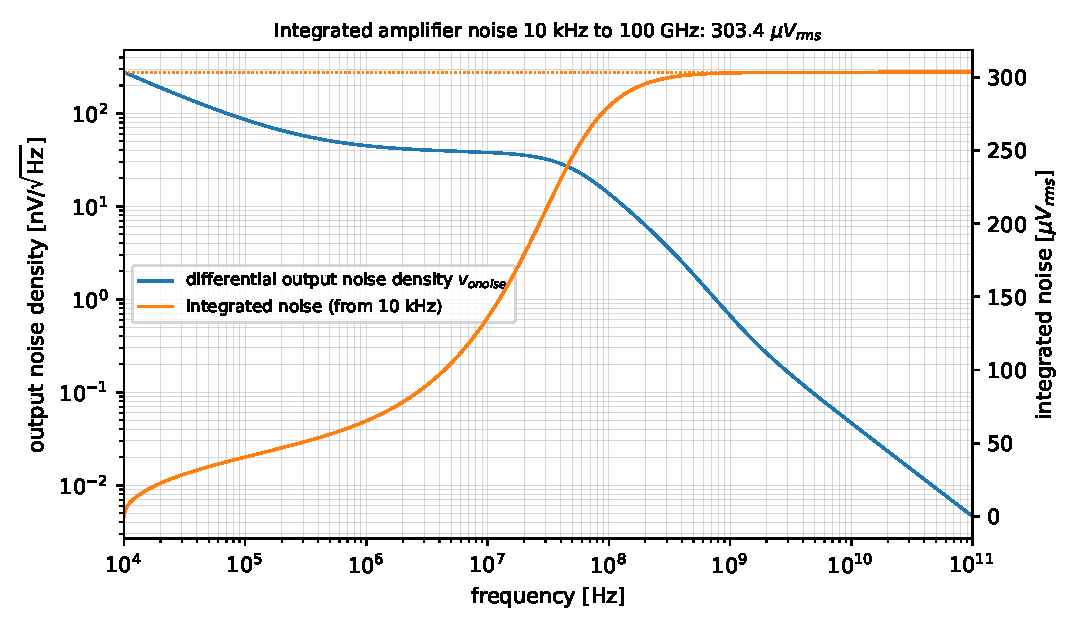
\includegraphics[width=\linewidth]{figures/d5_noise.pdf}}{\textcolor{red}{\textbf{?? missing figures/d5\_noise.pdf}}}
\caption{Differential output noise density from 10\,kHz to 100\,GHz and its running integral. Integrated
amplifier noise $\resVnAmp\,\mu$V$_{rms}$; with $kT/C$ ($\resKTC\,\mu$V$_{rms}$) the total is
$\resVnTot\,\mu$V$_{rms}$, SNR $= \resSNR$\,dB.}
\end{figure}
\clearpage

%% ---------------------------------------------------------------- page 7: D6
\section*{Deliverable 6: Difference in FoM between EE4520 and EE4525}
Both projects use $\mathrm{FoM_{lin}} = 2\pi P\tau/\mathrm{SNR_{lin}}^2$, so in decibels
$\mathrm{FoM_{dB}} = \mathrm{SNR_{dB}} - 10\log_{10}(2\pi P\tau)$. That makes the difference easy to take apart into a power
term, a time-constant term and an SNR term.

\textbf{Step 0, a fair baseline.} The EE4520 numbers need one correction first. That design (gain 8,
$C_{in} = C_{load} = 18$\,pF, $C_{fb} = 2.25$\,pF, 1.2\,V output step, no 1/f noise in the model, ideal CMFB and boosters)
reached $P = \ePow$\,mW and $\tau = \eTau$\,ns, measured between 40 and 48.69\,dB. Its SNR of \eSNR\,dB counted only the
integrated amplifier noise (76.93\,$\mu$V), with no $kT/C$, and its report put the 80.64\,dB specification into
$\mathrm{FoM_{lin}}$: 175.20\,dB, or \dd{\eFoM{\eSNR}}\,dB with the achieved SNR. EE4525 does include $kT/C$. The same rule
applied to the EE4520 network, $v_n^2 = 2kT(C_{in}/C_{fb}^2 + 1/C_{fb} + 1/C_{load})$, adds \dd[0]{\eKTC*1e6}\,$\mu$V. That
brings its SNR down to \dd{\eSNRll}\,dB and its FoM to \dd{\eFoM{\eSNRll}}\,dB, which is the value I compare against.

\begin{table}[H]\centering
\renewcommand{\arraystretch}{1.15}
\begin{tabular}{l r r r r}
\toprule
 & EE4520 (no $kT/C$) & EE4520 (with $kT/C$) & EE4525 & effect on $\mathrm{FoM_{dB}}$ \\
\midrule
Power $P$ [mW] & \ePow & \ePow & \resPower & $\dd{-10*\lgt{\resPower/\ePow}}$\,dB \\
$\tau$ [ns] & \eTau & \eTau & \resTau & $+\dd{-10*\lgt{\resTau/\eTau}}$\,dB \\
SNR [dB] & \eSNR & \dd{\eSNRll} & \resSNR & $\dd{\resSNR-\eSNRll}$\,dB \\
\midrule
$\mathrm{FoM_{dB}}$ [dB] & \dd{\eFoM{\eSNR}} & \dd{\eFoM{\eSNRll}} & \resFoMdB & $+\dd{\resFoMdB-\eFoM{\eSNRll}}$\,dB \\
\bottomrule
\end{tabular}
\end{table}

\textbf{Step 1, power ($\dd{-10*\lgt{\resPower/\ePow}}$\,dB).} EE4525 uses $\dd{\resPower/\ePow}\times$ more power. It
has to settle to 66\,dB accuracy in 25\,ns with every block built from transistors, the CMFB amplifier now draws from
$V_{dd}$, and the class-AB output supplies the load charge during the step (\xIslew\,$\mu$A of the \xIwin\,$\mu$A window
average).

\textbf{Step 2, time constant ($+\dd{-10*\lgt{\resTau/\eTau}}$\,dB).} $\tau$ is $\dd[0]{\eTau/\resTau}\times$ shorter, so
the energy spent per time constant, $P\tau$, falls from \dd[1]{\ePow*\eTau}\,pJ to \dd[3]{\resPower*\xTauExact}\,pJ.

\textbf{Step 3, SNR ($\dd{\resSNR-\eSNRll}$\,dB).} Only 66\,dB is needed, so the capacitors are about ten times smaller
($C_{in} = \resCin$\,pF) and the SNR is lower.

\textbf{Why the FoM ends up higher.} Take $P \propto I$, $\tau \propto C_{L,eff}/(\beta g_m)$ and, for $kT/C$-limited
sampling, $\mathrm{SNR_{lin}}^2 \propto V_{sig}^2 C_{in}/(N_{net}kT)$. The capacitance then cancels:
\[
\mathrm{FoM_{lin}} \propto \frac{C_{L,eff}}{C_{in}}\cdot\frac{N_{net}\,kT\,V_{DD}\,(I/g_m)}{\beta V_{sig}^2}.
\]
The SNR target itself does not
move the FoM, so the like-for-like gain of $+\dd{\resFoMdB-\eFoM{\eSNRll}}$\,dB has to come either from the test circuit or
from the amplifier. The test circuit explains most of it. The gain-4 network has a $kT/C$ noise gain
$N_{net} = 2(G^2+G+1)$ of 42 instead of 146 $kT/C_{in}$ ($\dd{10*\lgt{146/42}}$\,dB), an ideal feedback factor of 0.2
instead of $1/9$ ($\dd{10*\lgt{0.2*9}}$\,dB), and a slightly worse $C_{L,eff}/C_{in}$ of 1.20 instead of 1.11
($\dd{-10*\lgt{1.2/(1+1/9)}}$\,dB). My larger swing (\dd[1]{\resVout}\,V against 1.2\,V) adds
$\dd{20*\lgt{\resVout/1.2}}$\,dB. The $\tau$ definition is worth another $\dd{10*\lgt{\xTauTail/\xTauExact}}$\,dB: here
$T_{30}$ to $T_{38.6}$ lands in the fast stretch right after slewing, while the small-signal tail decays with
$\tau \approx \xTauTail$\,ns, and EE4520 measured $\tau$ in its linear tail. What remains,
$\dd{\resFoMdB-\eFoM{\eSNRll} - 10*\lgt{146/42} - 10*\lgt{0.2*9} + 10*\lgt{1.2/(1+1/9)} - 20*\lgt{\resVout/1.2} - 10*\lgt{\xTauTail/\xTauExact}}$\,dB,
is the circuit itself ($I/g_m$ and noise factor). Most of it comes from the complementary input pair, which gives twice
the $g_m$ per ampere and has no load devices adding noise. Current-buffer compensation and the class-AB output help as
well, with fast non-dominant poles and slewing current that is not paid for in quiescent current. Against that, the real
CMFB costs \opI{mct}, the 1/f noise now in the model takes \xFlickShare\,\% of the amplifier noise power, and the slewing
charge is counted in the 25\,ns power window.
\clearpage

%% ---------------------------------------------------------------- page 8: short explanation
\section*{Short Explanation}
\small
\textbf{Settling plot (D4).} At the step the output has not moved yet, so $A\beta$ starts at 0\,dB. The virtual-ground
error starts at $\beta_{act}V_{out,step}$, which puts $A$ \resGapdB\,dB higher. The input edge also couples through $C_{fb}$
and $C_c$ and first kicks the output \xKick\,mV the wrong way, so $A\beta$ dips to $\xAbDip$\,dB before it rises. The gap is
larger than the ideal 13.98\,dB, as it should be: the input pair adds $C_p \approx \xCp$\,fF at the summing node, so
$\beta_{act} = C_{fb}/(C_{in}+C_{fb}+C_p) = \resBetaActual$ sits below $C_{fb}/(C_{in}+C_{fb}) = \resBetaIdeal$.
At first both curves rise slowly. The input error ($\approx\dd{\resBetaActual*\resVout}$\,V) is beyond the linear range of
the input pairs, so stage 1 pushes its full tail current into $C_c$ and the outputs slew. Once the loop leaves slewing both
curves climb steeply. $T_{30}$ and $T_{38.6}$ fall in this stretch, so $\tau = \resTau$\,ns describes the fast transition.
The small-signal tail after it is slower ($\tau \approx \xTauTail$\,ns, fitted from 16 to 24\,ns), though still faster than
$1/(2\pi f_c) = \dd{1e3/(2*pi*\xFc)}$\,ns: with $\xPM^\circ$ of phase margin the non-dominant poles push the dominant
closed-loop pole above $f_c$. Finally the curves level off at floors set by the loop gain at the settled
$\pm\fpeval{\resVout/2}$\,V outputs ($A\beta$ \xAbEnd\,dB, $A$ \xAEnd\,dB at \xTend\,ns). These are above the DC $A_0\beta$
there (\xTzeroExt\,dB; \xTzero\,dB balanced) because within the window the AC-coupled output PMOS adds its $g_m$. The gap
grows from \resGapdB\,dB to $\dd{\resA-\resAbeta}$\,dB at 25\,ns and $\dd{\xAEnd-\xAbEnd}$\,dB at \xTend\,ns. At low
frequency the input-device drains carry $v_1$ divided by the cascode gain; in the 1\,kHz loop bench they swing \xMillNa\
(NMOS) and \xMillNb\ (PMOS) times the virtual-ground error, since the NMOS cascode has little gain at its small $V_{ds}$.
In the slow tail $C_{gd}$ is therefore Miller-multiplied and the effective $C_p$ grows. The error never changes sign, so
there is no ringing peak anywhere in the simulated window.

\textbf{Architecture and CMFB.} Two stages give enough gain without boosters, which would cost current. Stage 1 is a
stacked complementary pair (a PMOS pair on a top tail, an NMOS pair on a bottom tail, both driven by the summing node) with
PMOS and NMOS cascodes. The same current produces both $g_m$'s, so the stage needs half the current for its $g_{m1}$ and
has no load devices adding noise. Stage 2 is class-AB: $v_1$ drives the NMOS directly and the PMOS through $C_{ls}$, whose
DC level comes from $v_{bo}$ through $R_b$, so slewing current is not limited by the quiescent current. For compensation I
used current buffers, with $C_c$ split between the NMOS- and PMOS-cascode sources. There is no right-half-plane zero and no
nulling resistor, and the output stage needs little current ($f_c = \xFc$\,MHz, PM $\xPM^\circ$). The CMFB is
continuous-time. It senses the output CM with \pRcm\,M$\Omega \parallel C_{CM}$, compares it with $v_{cmr}$ in a PMOS pair
and corrects part of the NMOS tail ($M_{tc}$) through a diode mirror. Its loop crosses over at \xCMfc\,MHz with
\xCMpm$^\circ$ margin, the output CM sits at \xVcm\,V, and the CM bump during slewing is \xCMexc\,mV (\xCMexcTf\,mV at
25\,ns). It needs no clocks, and the sense network is all it adds to the outputs.

\textbf{Sizing.} I fixed the swing first. The outputs hold $\pm\fpeval{\resVout/2}$\,V with every transistor saturated, so
$V_{out,step} = \fpeval{round(\resVout,2)}$\,V; more swing collapses $A_0$ at the extremes. Of the noise power, $kT/C$
($42kT/C_{in}$) is \dd[0]{100*\resKTC^2/(\resKTC^2+\resVnAmp^2)}\,\% and the amplifier
\dd[0]{100*\resVnAmp^2/(\resKTC^2+\resVnAmp^2)}\,\%. The amplifier term is roughly $\alpha kT/C_c$, with
$\alpha \approx 2\gamma(1+n)/\beta$ plus 1/f and cascode terms; $n$, the load-to-input $g_m$ ratio, is close to zero
here. $C_{in} = \resCin$\,pF and $C_c = \pCc$\,pF trade noise against stage-1 current ($g_{m1} \propto C_c$ for a given
$f_c$) and against slewing charge ($\propto C_{in}$), and I set them together with the bias currents in a constrained
power minimisation. For settling, the input devices run at $g_m/I_D \approx \xGmIdN$ (\xIdIn\,$\mu$A each), which gives
$g_{m1} = \xGmOne$\,mS per side and $f_c = \beta_{act} g_{m1}/(2\pi C_c) = \dd[1]{\resBetaActual*\xGmOne e-3/(2*pi*\pCc e-12)/1e6}$\,MHz.
$C_{ls}$, $C_{1d}$ and the output quiescent current then set the damping, so the response is fast but never overshoots.
The 1/f noise is \xFlickShare\,\% of the amplifier noise power (\xFlickUV\,$\mu$V). In \texttt{log018.l} the NMOS flicker
spectrum falls only as $1/f^{0.825}$ (PMOS $1/f^{1.25}$) and reaches well into the band, so I gave the NMOS inputs
$L = 1\,\mu$m (\xFlickN\,$\mu$V each) and kept the PMOS inputs at 0.25\,$\mu$m (\xFlickP\,$\mu$V each) to limit $C_p$.

\textbf{Noise devices and NEF.} The four input transistors produce \xNinShare\,\% of the amplifier noise power
($M_{1n}$, $M_{2n}$: \xNinN\,$\mu$V each; $M_{1p}$, $M_{2p}$: \xNinP\,$\mu$V each). The cascodes come next (\xNcasN\ and
\xNcasP\,$\mu$V). Using $v_{n,amp}^2 = \mathrm{NEF}\cdot 2kT/(\beta C_{L,eff})$ with
$C_{L,eff} = C_{load} + (1-\beta)C_{fb} = \resCLeff$\,pF and $\beta = \resBetaIdeal$ gives NEF $= \resNEF$.

\textbf{Biasing.} A separate block on $V_{ddb}$, not counted in the power, turns ideal reference currents into gate
voltages. All the currents are fixed multiples of $I_b = \pIb\,\mu$A. The tails and the output PMOS are mirrored from
diode-connected replicas with the same $L$, and the cascode gates $v_{cn}$ and $v_{cp}$ come from long-$L$ diodes. Every
bias line is decoupled by $C_{big} = \resCbig$\,nF. The CMFB sets the rest of the NMOS tail. Power is 1.8\,V times the
larger of the quiescent current and the average over the 25\,ns amplification window.
\normalsize
\end{document}
